% TO DO: add citations in thesis work, better research plan

\documentclass[10pt]{beamer}
\usetheme[height=0mm]{Rochester}
\usecolortheme{}
\usefonttheme[onlylarge]{structurebold}
\setbeamerfont*{frametitle}{size=\normalsize,series=\bfseries}
\setbeamertemplate{navigation symbols}{}
\setbeamercovered{dynamic}
\setbeamertemplate{itemize item}[triangle]
\setbeamertemplate{itemize subitem}[triangle]

%  use Darmstadt if commenting the next line
\usepackage[footheight=1em]{beamerthemeboxes}
\usepackage[natbib=true,backend=biber,citestyle=authoryear]{biblatex}
\bibliography{../bib/stats}

\definecolor{bleu}{rgb}{0.2,0.4,0.65}
\setbeamercolor{palette primary}{bg=bleu,fg=white}
\setbeamercolor{palette secondary}{bg=bleu,fg=white}
\setbeamercolor{palette tertiary}{bg=bleu,fg=white}
\setbeamercolor{palette quaternary}{bg=bleu,fg=white}
\setbeamercolor{structure}{fg=bleu} % itemize, enumerate, etc
\setbeamercolor{section in toc}{fg=bleu} % TOC sections

\let\oldcite=\cite
\renewcommand\cite[1]{\hyperlink{#1}{\textcolor{vert}{\oldcite{#1}}}}
\let\oldcitep=\citep
\renewcommand\citep[1]{\hyperlink{#1}{\textcolor{vert}{\oldcitep{#1}}}}

\usepackage{amsmath,amssymb,amsthm,bbm}             % AMS Math
\usepackage[utf8]{inputenc}
\usepackage[english]{babel}
\usepackage{xcolor}
\usepackage{graphicx}
\usepackage{myAlgorithm}
\usepackage{subfigure}
\usepackage{hyperref}
\usepackage{mathtools}
\usepackage{mathrsfs}
\usepackage{cancel}
% commands
\def\onefig{.9\textwidth}
\def\twofig{0.48\textwidth}
\def\threefig{.26\textwidth}
\def\twofigplus{0.9\textwidth}
\definecolor{vert}{rgb}{0.1,0.55,0.35}
\definecolor{orange}{rgb}{1,0.5,0}
\definecolor{bleu}{rgb}{0.2,0.4,0.65}
\newcommand{\un}[1]{\textcolor{magenta}{#1}}
\newcommand{\unn}[1]{\textcolor{bleu}{#1}}
\newcommand{\unnn}[1]{\textcolor{orange}{#1}}
\newcommand{\unnnn}[1]{\textcolor{vert}{#1}}
\newcommand{\blank}{\vspace{.5\textheight}}
% notation
\def\i{\mathrm{i}}
\DeclareMathOperator*{\argmax}{arg\,max}
\DeclareMathOperator*{\argmin}{arg\,min}
\newcommand{\cA}{\mathcal{A}}
\newcommand{\cS}{\mathcal{S}}
\newcommand{\cF}{\mathcal{F}}
\newcommand{\cX}{\mathcal{X}}
\newcommand{\cY}{\mathcal{Y}}
\newcommand{\cZ}{\mathcal{Z}}
\newcommand{\cN}{\mathcal{N}}
\newcommand{\cO}{\mathcal{O}}
\renewcommand{\leq}{\leqslant}
\renewcommand{\geq}{\geqslant}
\renewcommand{\phi}{\varphi}
\renewcommand{\epsilon}{\varepsilon}
\renewcommand{\d}{ {\rm d}}
\renewcommand{\emptyset}{\varnothing}

\usepackage{tikz}
\usetikzlibrary{bayesnet}
\usetikzlibrary{arrows}
\usepackage{url}

\def\tpi{\widetilde{\pi}}
\def\figdir{Figures}

\setbeamertemplate{footline}[frame number]

\AtBeginSection[] % Do nothing for \section*
{
\begin{frame}
\frametitle{Outline}
\tableofcontents[currentsection]
\end{frame}
}

\newcommand{\backupbegin}{
   \newcounter{framenumberappendix}
   \setcounter{framenumberappendix}{\value{framenumber}}
}
\newcommand{\backupend}{
   \addtocounter{framenumberappendix}{-\value{framenumber}}
   \addtocounter{framenumber}{\value{framenumberappendix}}
}
\makeatletter

\title[Bayesian ML: Bayesics]{BML lecture \#2: MCMC}
\subtitle{\url{http://github.com/rbardenet/bml-course}}
\author[Rémi Bardenet (CNRS \& Univ. Lille)] % (optional, for multiple authors)
{Rémi Bardenet}
\institute[] % (optional)
{
  CNRS \& CRIStAL, Univ. Lille, France\\
\vspace{1cm}
\includegraphics[width=0.15\textwidth]{/Users/rbardenet/Work/Tex/PosterImages/logoCNRS.pdf}
\qquad \includegraphics[width=0.4\textwidth]{/Users/rbardenet/Work/Tex/PosterImages/cristalLogo.pdf}
}
\date{}

\begin{document}
\begin{frame}
\maketitle
\end{frame}

\begin{frame}
\frametitle{Outline}
\tableofcontents
\end{frame}

%%%%%%%%%%%%%%%%%%%%%%
\section{Introduction}
%%%%%%%%%%%%%%%%%%%%%%

\begin{frame}{What comes to $your$ mind when you hear "Monte Carlo"?}
\end{frame}

\begin{frame}{Expected utility requires computing integrals}
  \begin{block}{Minimizing the posterior expected loss}
  If $\cA= \{a_g\}$ and we partition $s=(s_{\text{obs}}, s_{\text{u}})$, then, given $s_\text{obs}$, we choose
  $$
  g^\star(s_\text{obs}) = \argmin_{a\in\mathcal{A}} \un{\mathbb{E}_{s_{\text{u}}\vert s_{\text{obs}}} L(a,s)}.
  $$
\end{block}

  \begin{alertblock}{The bottleneck is computing integrals w.r.t. the posterior}
  \begin{itemize}
    \item E.g. for binary prediction with 0-1 loss
    $$
    y^\star \in \argmax_{y\in\{0,1\}} \int p(y\vert x,\theta) p(\theta\vert x_{1:n}, y_{1:n}) \d\theta
    $$
    \item or for estimation with squared loss
    $$
    \theta^\star = \int \theta p(\theta\vert y_{1:n}) \d\theta.
    $$
  \end{itemize}
\end{alertblock}
\end{frame}

\begin{frame}{Numerical integration}
  Let $\pi$ be a pdf w.r.t. $\d \theta$.

  \begin{block}{The problem of numerical integration}
    Find $T$ nodes
    $(\theta_t)$ and weights $(w_t)$ so that
    $$
    \int f(\theta)\pi(\theta)\d \theta \quad\approx\quad \sum_{t=1}^N w_t f(\theta_t), \quad \forall
    f\in\mathcal C,
    $$
    where $\mathcal C$ is a large class of functions.
  \end{block}
  \begin{alertblock}{A constraint for Bayesians: $\pi$ is only known up to a constant}
    E.g. in estimation,
    $$ \pi(\theta) = p(\theta\vert y_{1:n}) \propto p(y_{1:n}\vert\theta) p(\theta) =: \pi_u(\theta).$$
    Or in classification/regression,
    $$
    \pi(\theta) = p(\theta\vert x_{1:n}, y_{1:n}) \propto p(y_{1:n}\vert x_{1:n}, \theta) p(\theta)=: \pi_u(\theta).
    $$
  \end{alertblock}

  % \begin{exampleblock}{Main families of methods}
  %   \begin{itemize}
  %   \item variants of Riemann integration \cite{DaRa84},
  %   \item Gaussian quadrature \cite{Gau04},
  %   \item quasi-Monte Carlo methods \cite{DiKuSl13},
  %   \item \un{Monte Carlo methods \cite{RoCa04}: importance sampling, MCMC.}
  %   \end{itemize}
  % \end{exampleblock}
  \end{frame}

\begin{frame}{Riemann-like integration is impractical when $d\gg 1$.}
\blank
\begin{itemize}
\item For modern developments, see quasi-Monte Carlo integration \cite{DiPi10}.
\end{itemize}
\end{frame}

\section{Monte Carlo methods}
\begin{frame}{Monte Carlo integration}
\begin{block}{The Monte Carlo principle}
Find a distribution on $\theta_1,\dots,\theta_T$ and weights $w_t$ such that
$$ \un{\mathcal{E}_T(f) =  \sum_{t=1}^T w_t f(\theta_t) - \int f(\theta)\pi(\theta)\d \theta}$$
is small (with large probability, in quadratic mean, converges in law at some rate, etc.)
\end{block}
\begin{itemize}
  \item If you knew how to sample from $\pi$, you could take $\theta_t\sim\pi$ i.i.d., $w_t=1/T$, and prove e.g.
  $$ \mathbb{P}\left( \un{\mathcal{E}_T(f)} \geq \alpha\frac{\sigma(f)}{\sqrt{T}} \right) \leq \frac{1}{\alpha^2}, \quad \forall \alpha,$$
  as soon as $\sigma(f)^2 := \mathbb{V}_\pi [f(\theta) - \int f(\theta)\pi(\theta)\d\theta]<+\infty$.
\end{itemize}
\end{frame}

\begin{frame}{Self-normalized importance sampling}
\begin{itemize}
  \item Let $\pi_u(\theta) = Z\pi(\theta)$ be the unnormalized target pdf.
  \item Sample $\theta_{1:T}$ i.i.d. from $q$, and take
  $$
  w_t = \frac{\pi_u(\theta_t)}{q(\theta_t)} \times \left( \sum_{t=1}^T \frac{\pi_u(\theta_t)}{q(\theta_t)} \right)^{-1}
  $$
  so that $\sum w_t = 1$.
  \item Then
  \vspace{2cm}
  \item One can show that $ \sqrt{T}\un{\mathcal{E}_T(f)} \rightarrow \cN(0, \sigma^2_{\text{NIS}}(f))$.
  \item Problem is that for reasonable choices of $f,q,\pi$, \un{$\log \sigma_{\text{NIS}}(f) \propto d$}.
\end{itemize}
\vfill
\end{frame}

\section{The Metropolis-Hastings algorithm}

\begin{frame}{(Mostly) friendly faces}
\begin{figure}
  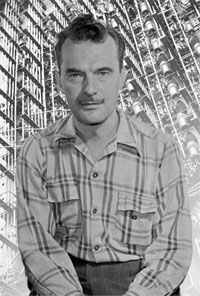
\includegraphics[height=.3\textheight]{Figures/metropolis}
  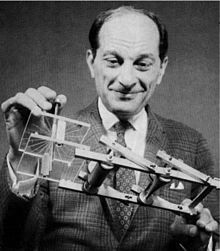
\includegraphics[height=.3\textheight]{Figures/ulam}\\
  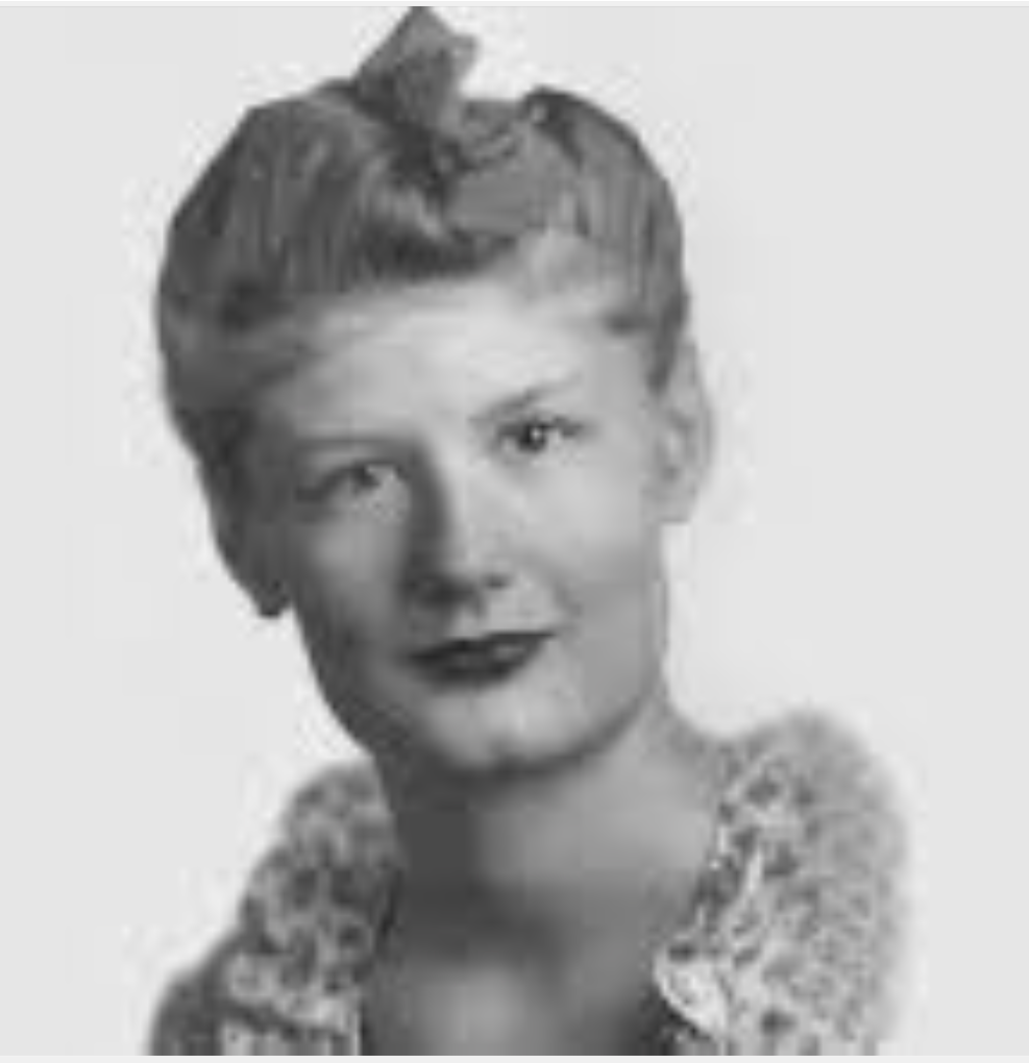
\includegraphics[height=.3\textheight]{Figures/rosenbluth}
  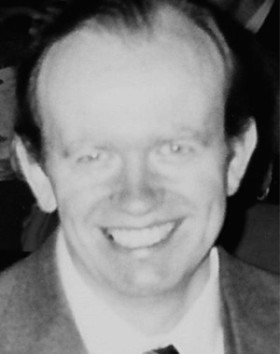
\includegraphics[height=.3\textheight]{Figures/hastings}
  \caption{A few MCMC pioneers: N. Metropolis, S. Ulam, A. Rosenbluth, W. K. Hastings}
\end{figure}\end{frame}

\begin{frame}{Markov chain Monte Carlo (MCMC; \citep{RoCa04})}
\begin{itemize}
  \item The idea is to take $(\theta_t)$ to be an ergodic Markov chain with limiting distribution $\pi$, so that for $f\in L^1(\pi)$,
  % $$
  % \lim \frac{1}{T} \sum_{t=1}^T f(\theta_t) \rightarrow \int f(\theta)\pi(\theta)\d\theta, a. s..
  % $$
  $$$$
  \vfill
  \item In MCMC research, when a new Markov kernel comes out, we typically first prove a \un{law of large numbers}, and then a \un{central limit theorem}, i.e., that under weak conditions on $\pi$ and $f$,
  % $$
  % \lim \sqrt{T}\mathcal E_T(f)  \rightarrow \cN(0,\sigma^2(f)),
  % $$
  $$$$
  \vfill
  and that $\sigma^2(f)$ can be estimated; see \citep{DoMoSt14}.
  \end{itemize}
\end{frame}

\begin{frame}{A law of large numbers for Markov chains}
  Let $(\theta_t)_{t\in\mathbb N}$ be a Markov chain on $\Theta$, with Markov kernel $P$. If
  \begin{itemize}
    \item There exists $\pi$ s.t. 
    $$
    \int \d\pi(x) P(x, B) = \pi(B).
    $$
    \item For any $A$ with $\pi(A)>0$, for any $\theta\in \Theta$,
    $$ 
    \mathbb{P}_{\theta} \left(\sum_{t=0}^\infty 1_{\theta_t\in A} = +\infty\right) = 1,
    $$
  \end{itemize}
  then for any $f$ such that $\int \vert f\vert \mathrm{d} \pi <\infty$, for any initial distribution $\mu_0$ of $\theta_0$, almost surely
  $$
  \frac{1}{T} \sum_{t=1}^T f(\theta_t) \rightarrow \int f\mathrm{d}\pi.
  $$
  See e.g. \citep{DoMoSt14}.
\end{frame}

\begin{frame}
\frametitle{The Metropolis-Hastings algorithm}
\begin{algorithm}{$\Algo{MH}\big(\unn{\pi_u},\, q(\cdot\vert\cdot),\,\theta_{0},\, T\big)$}
\Aitem \For $t\setto1$ \To $T$
\Aitem \mt $\theta\setto\theta_{t-1}$
\Aitem \mt $\theta'\sim \un{q(.\vert\theta)}$, $u\sim\mathcal U_{(0,1)}$,
\Aitem \mt $\rho =  \unn{\frac{\pi(\theta')}{\pi(\theta)}} \un{\frac{q(\theta\vert\theta')}{q(\theta'\vert\theta)}}$.
\Aitem \mt \If $u<\rho$,
\Aitem \mtt $\theta_{t}\setto\theta'$
\mt \algoremark{\unn{Accept}}
\Aitem \mt \Else $\theta_{t}\setto\theta$
\mt \algoremark{\unn{Reject}} \label{ai:acceptanceEnd}
\Aitem
\Return $(\theta_{t})_{t=1,\dots,N_{\text{iter}}}$
\end{algorithm}
\end{frame}

\begin{frame}{The MH Markov kernel...}
... is given by
  $$
P_{\text{MH}}(\theta,\theta') = \unnnn{\alpha(\theta,\theta')} \un{q(\theta'\vert\theta)} + \delta_\theta(\theta')\left[1-\int \unnnn{\alpha(\theta,\vartheta)}\un{q(\vartheta\vert\theta)}\right]\d\vartheta,
$$
where
$$
\unnnn{\alpha(\theta,\theta')} = 1\wedge \frac{\pi(\theta')}{\pi(\theta)} \un{\frac{q(\theta\vert\theta')}{q(\theta'\vert\theta)}}.
$$
\blank
\end{frame}

\begin{frame}{MH leaves $\pi$ invariant and satisfies the LLN}
\begin{itemize}
  \item We first show detailed balance, i.e., $\pi(\theta)P(\theta,\theta') = \pi(\theta')P(\theta',\theta).$
  \vfill
  \vfill
  \vfill
  \vfill
  \item We deduce that $P$ leaves $\pi$ invariant.
  \vfill
  \vfill
  \vfill
  \vfill
\end{itemize}
\vfill
\begin{block}{Theorem \citep{RoCa04}}
  If $\pi(A)>0\Rightarrow (\forall x) q(A\vert x)>0$, then $P_{\text{MH}}$ satisfies the LLN.
\end{block}
\begin{exampleblock}{Some additional useful properties}
  \begin{itemize}
    \item Note that if $P_1$ and $P_2$ leave $\pi$ invariant, then so does
    $$
    P_1P_2 (\theta,\theta') = \int P_1(\theta,\vartheta)P_2(\vartheta,\theta')\d\vartheta.
    $$
    \item The MH error scales polynomially with the dimension; see \href{https://statisfaction.wordpress.com/2018/05/15/scaling-of-mcmc-with-dimension-experiments/}{blog post}.
  \end{itemize}
\end{exampleblock}
\end{frame}

\section{Gibbs sampling}
\begin{frame}{The random scan Gibbs sampler}
\begin{itemize}
\item Consider MH with
$$
q(\theta'\vert\theta) = \frac1d \sum_{k=1}^d \un{\pi(\theta'_k\vert \theta_{\setminus k})} 1_{\theta'_{\setminus k} = \theta_{\setminus k}}, \quad \theta_{\setminus k}:= (\theta_1,\dots,\theta_{k-1},\theta_{k+1},\dots,\theta_d).
$$
\item Then the probability of acceptance $\alpha(\theta,\theta')$ is always $1$.
\vspace{2cm}
\vfill
\item In practice, the systematic scan Gibbs sampler is more common, which consists in repeatedly: drawing $\theta_1\vert\theta_{\setminus 1}$, then $\theta_2\vert\theta_{\setminus 2}$, etc. always conditioning on the newest values available of each $\theta_k$.
\item You can also partition $\theta$ in arbitrary blocks.
\end{itemize}
\end{frame}

\begin{frame}{An example: Latent Dirichlet allocation}
\centering
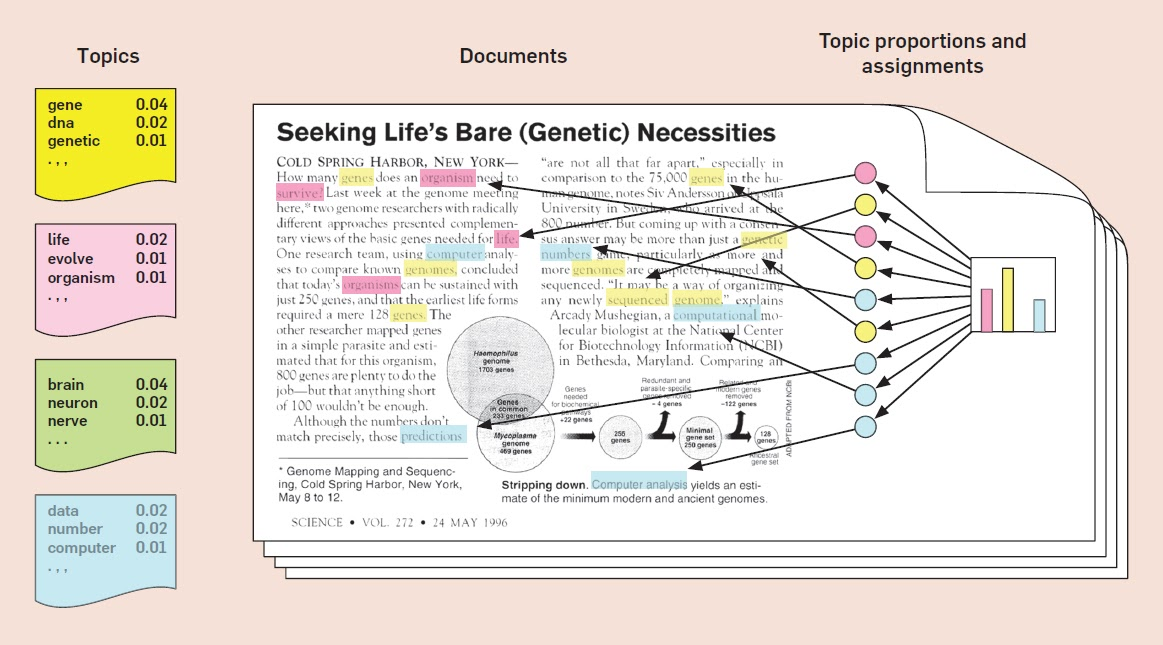
\includegraphics[width=.9\textwidth]{\figdir/lda.jpg}
\vfill
\end{frame}

\begin{frame}{A Gibbs sampler for LDA}

\end{frame}

\begin{frame}{Collapsed Gibbs sampling for LDA}

\end{frame}

\section{Hamiltonian Monte Carlo}

\begin{frame}{An abstract variant of MH}
\begin{itemize}
  \item Let $S$ be a linear involution of $\cX\subset\mathbb{R}^{2d}$, such that $\eta\circ S = \eta$ for some (possibly unnormalized) PDF $\eta$.
  \vspace{2.5cm}
  \item Let further $\Phi:\mathbb{R}^{2d}\rightarrow \mathbb{R}^{2d}$ be a $C^1$-diffeomorphism such that $S\circ \Phi = \Phi^{-1}\circ S$.
  \item Now let 
\begin{equation}
    \label{e:acceptance_probability_abstract_HMC}
    \alpha(x) \triangleq 1\wedge \frac{\eta(\Phi(x))}{\eta(x)} \vert\Phi'(x)\vert,
\end{equation}
and consider the Markov kernel
$$
P_{aHMC}(x,A) = \alpha(x) 1_{\Phi(x)\in A} + (1-\alpha(x))1_{S(x)\in A}.
$$
\end{itemize}
\begin{block}{Proposition}
$P_{aHMC}$ leaves $\eta$ invariant.
\end{block}
\end{frame}

\begin{frame}{Hamiltonian dynamics is the source of inspiration}
\begin{block}{Hamilton's equations of motion}
Consider a physical system described by Hamiltonian $H(x,\xi)$ in phase space $(x,\xi)\in \mathbb{R}^{2d}$. Then the trajectories are prescribed by
\begin{equation}
  \label{e:hamilton}
  \dot{x_i} = \frac{\partial H}{\partial \xi_i} \qquad \dot{\xi_i} = -\frac{\partial H}{\partial x_i}.
\end{equation}
\end{block}
\begin{itemize}
  \item Given an initial point $(x,\xi)$, solve \eqref{e:hamilton} and denote the corresponding position in $\mathbb{R}^{2d}$ at time $t>0$ by $\Phi_t(x,\xi)$.
  \item \eqref{e:hamilton} implies that $t\mapsto H(\Phi_t(x,\xi))$ is constant.
  \item As an example, consider $H(x,\xi) = \frac12 x^2 + \frac12 \xi^2.$
\end{itemize}
\blank
% Describe, show Jacobian, show scaling with dimension, % discuss automatic differentiation and pymc3
\end{frame}

\begin{frame}{Numerical approximations of the Hamiltonian flow}
\begin{itemize}
  \item One idea would be to put some monotone function of the target in the Hamiltonian, such as $ H(q,p) = -\log \pi(q) + \frac12 \xi^T M \xi $.
  \item We know approximations of the Hamiltonian flow, such as the leapfrog (aka velocity Verlet) integrator. It is defined as $\psi_h^n = \psi_h \circ \dots \psi_h$, where $(p',q') = \psi_h(p,q)$ is 
\begin{align*}
    p_{1/2} &= p + \frac{h}{2}\nabla \log \pi(q)\\
    q' &= q+hM^{-1}p_{1/2}\\
    p' &= p_{1/2} + \frac{h}{2} \nabla \log\pi (q');
\end{align*}
\end{itemize}
\begin{block}{Proposition}
  The leapfrog integrator satisfies $S\circ \psi_h^n = (\psi_h^n)^{-1}\circ S$ for $S(q,p) = (q,-p)$, and $\vert \det (\psi_h^n)'(q,p)\vert = 1$. 
\end{block}
\end{frame}

\begin{frame}{Hamiltonian Monte Carlo mimics a physical system}
  \begin{itemize}
    \item Let $\log \tpi(x, \xi) =  \log \pi(x) + \frac12 \xi^T M(x) \xi$.
    \item Consider the Markov kernel $P((x,\xi), (x,\xi'))$ given by the product of
    $$ \xi\sim \cN(0,M(x)^{-1})$$
    and
    $$
    P_{aHMC}(x,A) = \alpha(x) 1_{\Phi(x)\in A} + (1-\alpha(x))1_{S(x)\in A}.
    $$
    where 
    \begin{equation}
      \alpha(x) \triangleq 1\wedge \frac{\tpi(\psi_h^n(x))}{\tpi(x)} \cancel{\vert (\psi_h^n)'(x))\vert},
    \end{equation}
    Then \un{$P$ leaves $\pi$ invariant}.
\end{itemize}
\blank
\end{frame}

% Show Chi Feng's demo.


\section{Convergence diagnostics for MCMC}
\begin{frame}{What can go wrong?}
\begin{figure}
\includegraphics[width=\textwidth]{Figures/cvDiagnostics}
\caption{Taken from \citep{GCSDVR13}}
\end{figure}
We need to monitor both cross-chain and within-chain behavior.
\end{frame}

\begin{frame}{Comparing $P$ chains with overdispersed starting points}
\begin{itemize}
  \item The behaviour of the $P$ traces should become similar.
  \item Always make visual sanity checks!
  \item Scalar estimates should converge to the same value.
  \item We can also compare the variance of a scalar estimate within- and across chains
\end{itemize}

  \begin{block}{The Gelman-Rubin diagnostic}
  \begin{itemize}
    \item Choose an $f$ of interest, e.g. $f(\theta) = \theta_1$.
    \item Compute $B:=\frac{T}{P-1}\sum_{p=1}^P (\bar f_{\cdot p} - \bar f_{\cdot\cdot})^2$.
    \item Compute $W:=\frac1P \sum_{p=1}^P\left[ \frac{1}{T-1} \sum_{t=1}^T (\bar f_{tp}-\bar f_{\cdot p})^2\right].$
    \item Then check whether
    $$\hat R = \sqrt{\frac{\un{\frac{T-1}{T}W + \frac1T B}}{\unnnn{W}}}\in[1,1.1].$$
    \item See \citep{VaKn21} for an insightful discussion.
  \end{itemize}
\end{block}
\end{frame}

\begin{frame}{More convergence diagnostics}
\begin{block}{Single-chain diagnostics}
  \begin{itemize}
  \item The idea is to compare different chunks of a single chain.
  \item At stationarity, large chunks should be statistically indistinguishable.
  \item The \un{Geweke diagnostic} tests this similarity \citep{Gew92}
  \end{itemize}
\end{block}

\begin{block}{Effective sample size}
  \begin{itemize}
  \item Autocorrelation in each chain is what increases the variance of scalar estimands, compared to i.i.d. draws from $\pi$.
  \item We can estimate this autocorrelation, and build an estimator for $PT$ times the ratio of the two variances $\widehat{ESS}\in [1,PT]$, called, the \un{\emph{effective sample size}}; see Section 11.5 of \citep{GCSDVR13}.
  \item \cite{VaKn21} note that
  $$\hat R \approx \sqrt{1+P/\widehat{ESS}},$$ so $\hat R=1.1$ \un{only} corresponds to $\widehat{ESS}=5P$ .
  \end{itemize}
\end{block}
\end{frame}


\begin{frame}{Conclusion}
\begin{block}{Take-home message}
  \begin{itemize}
    \item MCMC approximates the integrals in the expected utility framework.
    \item Try to \un{leverage the problem's structure} to design your kernels.
    \item Otherwise, try standard kernels like HMC.
    \item Always monitor convergence.
  \end{itemize}
\end{block}

\onslide<2>
  \begin{itemize}
  \item HMC with NUTS is the default choice in most probabilistic programming frameworks.
  \item MCMC is a \un{rich research topic}. Some keywords: Wang-Landau, Langevin, equi-energy, hit-and-run, bouncy particle sampler.
  \item Besides Markov chains, checkout \un{sequential Monte Carlo samplers} \citep{DeDoJa06}.
  \item Deterministic methods are also investigated: \un{quasi-Monte Carlo methods} \citep{DiPi10} have the best convergence rates as soon as the integrand is smooth.
\end{itemize}
\end{frame}


\section*{References}
\setbeamertemplate{bibliography item}[text]%,
\begin{frame}[allowframebreaks]
\frametitle{References}
\small
\printbibliography
\normalsize
\end{frame}

\end{document}

% trail junk

\section{The what}

\subsection{Typical statistical problems}
\begin{frame}
\frametitle{Typical jobs for statisticians}
\begin{block}{Estimation}
\begin{itemize}
\item You have data $x_1,\dots,x_n$ that you assume drawn from $p(x_1,\dots,x_n\vert \theta^\star)$, with $\theta^\star\in\mathbb{R}^d$.
\item You want \un{an estimate $\hat{\theta}(x_1,\dots,x_n)$} of $\theta^\star\in\mathbb{R}^d$.
\end{itemize}
\end{block}
\uncover<2>{
\begin{block}{Confidence regions}
  \begin{itemize}
  \item You have data $x_1,\dots,x_n$ that you assume drawn from $p(x_1,\dots,x_n\cdot\vert \theta^\star)$, with $\theta^\star\in\mathbb{R}^d$.
  \item You want \un{a region $A(x_1,\dots,x_n)\subset \mathbb{R}^d$} and make a statement that $\theta\in A(x_1,\dots,x_n)$ with some certainty.
  \end{itemize}
\end{block}
}
\end{frame}

\subsection{Statistical decision theory}
\begin{frame}
\frametitle{Statistical decision theory\footcite{Wal50}}
\begin{figure}
  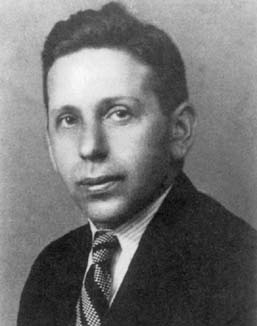
\includegraphics[width=\threefig]{\figdir/wald.jpg}
  \caption{Abraham Wald (1902--1950)}
\end{figure}
\end{frame}

\begin{frame}
\frametitle{Statistical decision theory}
\begin{itemize}
\item Let $\Theta$ be the ``states of the world", typically the space of parameters of interest.
\item Decisions are functions $d(x_1,\dots,x_n)\in \mathcal{D}$.
\item Let $L(d,\theta)$ denote the loss of making decision $d$ when the state of the world is $\theta$.
\item Wald defines the risk of a decision as
  $$ R(d,\theta) = \int L(d,\theta) p(x_{1:n}\vert \theta) \un{dx_{1:n}}.$$
\item Wald says $d_1$ is a \un{better} decision than $d_2$ if
\begin{equation}
  \un{\forall \theta\in\Theta,}\quad L(d_1,\theta)\leq L(d_2,\theta).
\label{e:waldOrder}
\end{equation}
\item $d$ is called \un{admissible} if there is no better decision than $d$.
\end{itemize}
\end{frame}

\begin{frame}
\frametitle{Illustration with a simple estimation problem}
\begin{itemize}
  \item You have data $x_1,\dots,x_n$ that you assume drawn from
  $$p(x_1,\dots,x_n\vert \theta^\star) = \prod_{i=1}^n \cN(x_i\vert\theta^\star,\sigma^2),$$ and you know $\sigma^2$.
  \item You \un{choose} a loss function, say $L(\hat{\theta},\theta) = \Vert \hat{\theta}-\theta\Vert^2.$
  \item You \un{restrict} your decision space to unbiased estimators.
  \item The sample mean $\tilde{\theta}:= n^{-1}\sum_{i=1}^n x_i$ is unbiased, and has minimum variance among unbiased estimators.
  \item Since $$R(\tilde\theta,\theta) = \text{Var}\tilde\theta,$$ $\tilde{\theta}$ is the \un{best decision} you can make in Wald's framework.
\end{itemize}
\end{frame}

\begin{frame}
  \frametitle{Wald's view of frequentist estimation}
  \begin{block}{Estimation}
  \begin{itemize}
  \item You have data $x_1,\dots,x_n$ that you assume drawn from $p(x_1,\dots,x_n\vert \theta^\star)$, with $\theta^\star\in\mathbb{R}^d$.
  \item You want \un{an estimate $\hat{\theta}(x_1,\dots,x_n)$} of $\theta^\star\in\mathbb{R}^d$.
  \end{itemize}
  \end{block}

\begin{exampleblock}{A Waldian answer}
\begin{itemize}
\item Our decisions are estimates $d(x_1,\dots,x_n) = \hat{\theta}(x_1,\dots,x_n)$.
\only<1>{
\item \un{We pick a loss}, say $L(d,\theta) = L(\hat{\theta},\theta) = \Vert \hat{\theta}-\theta\Vert^2$.
\item
If you have an unbiased estimator with minimum variance, then this is \un{the best decision among unbiased estimators}.
}
\only<2>{
\item In general, the loss can be more complex and unbiased estimors unknown/irrelevant.
\item In these cases, you may settle for a \un{minimax estimator}
$$ \hat\theta(x_1,\dots,x_n) = \argmin_d \sup_\theta R(d,\theta).$$
}
\end{itemize}
\end{exampleblock}
\end{frame}

\begin{frame}
\frametitle{Wald's is only \emph{one} view of frequentist statistics...}
\begin{itemize}
\item On estimation, some would argue in favour of the maximum likelihood \footcite{Sti07}.
\end{itemize}
\begin{figure}
  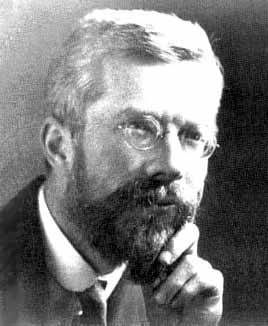
\includegraphics[width=\threefig]{\figdir/fisher.jpg}
  \caption{Ronald Fisher (1890--1962)}
\end{figure}
% In a sense, MLE is a limiting case of Wald's approach, but not clean
\end{frame}

\begin{frame}
\frametitle{... but bear with me, since it is predominant in machine learning}
For instance, supervised learning is usually formalized as
\begin{equation}
g^\star = \argmin_g \mathbb{E}L(y,g(x)).
\label{e:learning}
\end{equation}
which you approximate by
$$ \hat{g} = \argmin_g \sum_{i=1}^n L(y_i,g(x_i)) + \text{penalty}(g),$$
while trying to control the excess risk
$$ \mathbb{E}L(y,\hat g(x)) - \mathbb{E}L(y,g^\star(x)).$$
\end{frame}


\begin{frame}
  \frametitle{Wald's view of frequentist confidence regions}
  \begin{block}{Confidence regions}
    \begin{itemize}
    \item You have data $x_1,\dots,x_n$ that you assume drawn from $p(x_1,\dots,x_n\cdot\vert \theta^\star)$, with $\theta^\star\in\mathbb{R}^d$.
    \item You want \un{a region $A(x_1,\dots,x_n)\subset \mathbb{R}^d$} and make a statement that $\theta\in A(x_1,\dots,x_n)$ with some certainty.
    \end{itemize}
  \end{block}

\begin{exampleblock}{A Waldian answer}
\begin{itemize}
\item Our decisions are subsets of $\mathbb{R}^d$: $d(x_{1:n}) = A(x_{1:n})$.
\item A common loss is $L(d,\theta) = L(A,\theta) = 1_{\theta\notin A} + \gamma \vert A\vert $.
\item So you want to find $A(x_{1:n})$ that minimizes
$$ L(A,\theta) = \int \left[1_{\theta^\star\notin A} p(x_{1:n}\vert\theta^{\star}) + \gamma \vert A\vert\right] dx_{1:n} .$$
\end{itemize}
\end{exampleblock}
\end{frame}

\begin{frame}
\frametitle{Illustration with a simple confidence interval problem}
\begin{itemize}
  \item You have data $x_1,\dots,x_n$ that you assume drawn from
  $$p(x_1,\dots,x_n\vert \theta^\star) = \prod_{i=1}^n \cN(x_i\vert\theta^\star,\sigma^2).$$
  \item You \un{choose} a loss function, say $L(A,\theta) = 1_{\theta\notin A} + \gamma \vert A\vert $.
  \item You \un{restrict} your decisions to intervals centered around the sample mean $\tilde\theta$.
  \item Since $\frac{\theta - \tilde\theta}{\sigma/\sqrt{n}} \sim \cN(0,1)$,
  we know \unn{(exercise)} that for $$\tilde{A} := [\tilde\theta - k\sigma/\sqrt{n}, \tilde\theta + k\sigma/\sqrt{n}],$$
  it comes
  $$ R(A, \theta) = \mathbb{P}(\vert\cN(0,1)\vert \geq k) + \frac{2\gamma k\sigma}{\sqrt{n}}.$$
  \item All is left to do is choose $k$.
  \item Textbook examples bypass the need for $\gamma$: they fix $\alpha>0$ and find the smallest $k$ such that $\mathbb{P}(\vert\cN(0,1)\vert \geq k)\leq \alpha$.
\end{itemize}
\end{frame}

\begin{frame}
\frametitle{Summary so far}
% Maybe introduce a classification example here
\begin{itemize}
\item Waldian frequentists measure risks as expectations w.r.t. the data-generating process.
$$ R(d,\theta) = \int L(d(x_{1:n}),\theta) p(x_{1:n}\vert \theta)dx_{1:n}$$
\item One major difficulty is that the risk remains a function of $\theta$.
\item Without additional structure (unbiasedness, Gaussianity, etc.), it is difficult to go beyond minimax rules.
\end{itemize}
\begin{block}{Idea}
What if we introduced a distribution on $\Theta$, and tried to minimize
\begin{align*}
  r(d) &= \int R(d,\theta) p(\theta) \un{d\theta}\\
   &= \int\left[\int  L(d(x_{1:n}),\theta) p(x_{1:n}\vert \theta)dx_{1:n}\right]p(\theta)\un{d\theta}
\end{align*}
\end{block}
\end{frame}

\begin{frame}
\frametitle{From expected frequentist loss to posterior expected loss}
\begin{align*}
  r(d) &= \int R(d,\theta) p(\theta) \un{d\theta}\\
   &= \int\left[\int  L(d(x_{1:n}),\theta) p(x_{1:n}\vert \theta)dx_{1:n}\right]p(\theta)\un{d\theta}\\
   &\textcolor{red}{=} \int\left[\int  L(d(x_{1:n}),\theta) p(x_{1:n}\vert \theta)p(\theta)\un{d\theta} \right]dx_{1:n}\\
   &= \int\left[\int  L(d(x_{1:n}),\theta) \unn{\frac{p(x_{1:n}\vert \theta)p(\theta)}{p(x_{1:n})}}\un{d\theta} \right] p(x_{1:n}) dx_{1:n}\\
   &= \int\left[\int  L(d(x_{1:n}),\theta) \unn{p(\theta\vert x_{1:n})}\un{d\theta} \right] p(x_{1:n}) dx_{1:n}
\end{align*}
\end{frame}

\subsection{Posterior expected utility and Bayes rules}
\begin{frame}
\frametitle{Bayesians minimize posterior expected utility}
\begin{block}{The posterior expected utility paradigm: Bayes rules}
Pick $d$ to solve
$$ \argmin_d \int  L(d(x_{1:n}),\theta) p(\theta\vert x_{1:n}) d\theta. $$
\end{block}
\begin{exampleblock}{Bayes rules have good frequentist properties\footcite{PaIn09}}
\begin{itemize}
\item Under general conditions, Bayes decision rules are admissible, all admissible rules are limits of Bayes rules.
\item Bayes rules with ``least favourable priors" are minimax.
\end{itemize}
\end{exampleblock}
\end{frame}

\begin{frame}
  \frametitle{Illustration with a simple estimation problem}
  \begin{itemize}
    \item You have data $x_1,\dots,x_n$ that you assume drawn from
    $$p(x_1,\dots,x_n\vert \theta^\star) = \prod_{i=1}^n \cN(x_i\vert\theta^\star,\sigma^2),$$ and you know $\sigma^2$.
    \item You \un{choose} a loss function, say $L(\hat{\theta},\theta) = \Vert \hat{\theta}-\theta\Vert^2.$
    \item You \un{choose} a prior $p$ over $\theta$.
    \item Your Bayes decision minimizes
    $$ \int \Vert\hat{\theta}-\theta\Vert^2 p(\theta\vert x_{1:n})d\theta,$$
    so you pick
    $$ \hat\theta = \int \theta p(\theta\vert x_{1:n}) d\theta.$$
    \item Conceptually, it is simpler. In practice, you need to compute an integral.
  \end{itemize}
  \end{frame}

  \begin{frame}
  \frametitle{Illustration with a simple confidence interval problem}
  \begin{itemize}
    \item You have data $x_1,\dots,x_n$ that you assume drawn from
    $$p(x_1,\dots,x_n\vert \theta^\star) = \prod_{i=1}^n \cN(x_i\vert\theta^\star,\sigma^2).$$
    \item You \un{choose} a loss function, say $L(A,\theta) = 1_{\theta\notin A} + \gamma \vert A\vert $.
    \item You \un{choose} a prior $p$ over $\theta$.
    \item Your Bayes decision minimizes
    $$ \int 1_{\theta\notin A} p(\theta\vert x_{1:n})d\theta + \gamma\vert A\vert,$$
    \item Conceptually, it is simpler. In practice, you need to carefully pick your prior and/or restrict the decision space and/or compute many integrals.
  \end{itemize}
  \end{frame}

% \begin{frame}
%   \frametitle{Again, Wald's view is not universal}
%   \begin{center}
%   \includegraphics[width=\textwidth]{\figdir/stackexchange.png}
%   \end{center}
% \end{frame}

\begin{frame}
  \frametitle{Summary so far}
  \begin{itemize}
    \item Bayes rules fit into Wald's framework.
    \item \un{For a fixed prior}, the Bayesian risk completely orders decision rules.
    \item The \un{key idea} is posterior expected utility.
    \item You can answer most basic statistical questions using this principle: [more examples].
  \end{itemize}
\end{frame}

\begin{frame}
  \frametitle{A recent motivating success}
  \only<1>{
  \fbox{\includegraphics[trim={0 15cm 0 0},clip,width=\textwidth]{Papers/virgo.pdf}}
  }
\end{frame}


\section{The why}
\subsection{The philosophical why}

\begin{frame}
  \frametitle{The subjectivistic viewpoint}
  \begin{itemize}
    \item Top requirement is \un{internal coherence} of decisions.
    \item Favourizes interpreting probability distributions as personal beliefs.
    \begin{figure}
      \centering
      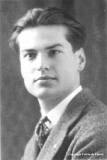
\includegraphics[width=\threefig]{\figdir/deFinetti.jpg}
      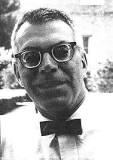
\includegraphics[width=\threefig]{\figdir/savage.jpg}
      \caption{Bruno de Finetti (1906--1985) and L. Jimmie Savage (1917--1971)}
    \end{figure}
  \end{itemize}
\end{frame}

\begin{frame}
  \frametitle{The logical justification}
  \begin{itemize}
    \item Top requirement is to find a version of propositional logic that allows taking into account uncertainty.
    \item Also favourizes interpreting \un{probability distributions as beliefs}, but aims for objective priors.
    \begin{figure}
      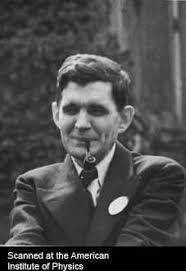
\includegraphics[width=\threefig]{\figdir/cox.jpg}
      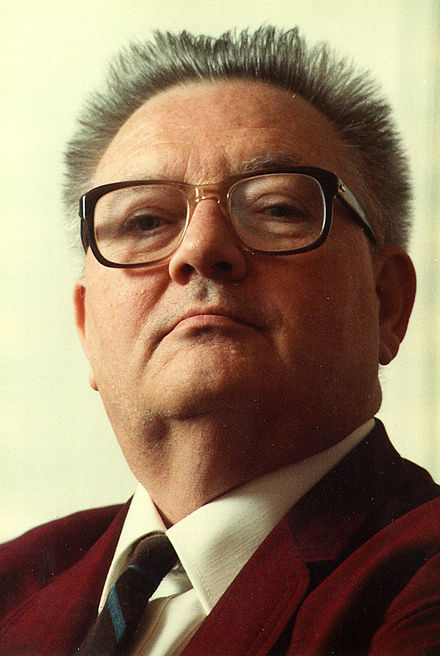
\includegraphics[width=\threefig]{\figdir/jaynes.jpg}
      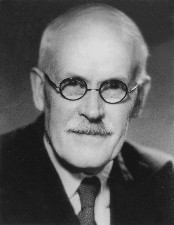
\includegraphics[width=\threefig]{\figdir/jeffreys.jpg}
      \caption{Richart T. Cox (1898--1991), Edwin T. Jaynes (1917--1971), and Harold Jeffreys (1891--1989)}
    \end{figure}
  \end{itemize}
\end{frame}

\begin{frame}
  \frametitle{The hybrid view\footcite{Rob07}}
  \begin{itemize}
    \item The starting point is posterior expected utility, loosely justified by Wald's theory.
    \item It is simple, widely applicable, has good frequentist properties.
    \item It satisfies the \un{likelihood principle}.
    \item It is easy to interpret: beliefs are
    \begin{itemize}
      \item represented by probabilities,
      \item updated using Bayes' rule,
      \item integrated when making decisions.
    \end{itemize}
    \item It is easy to communicate your uncertainty
    \begin{itemize}
      \item Simply give your posterior.
      \item When making a decision, make sure that the priors of everyone involved would yield the same decision.
    \end{itemize}
  \end{itemize}
\end{frame}

\subsection{The practical why}
\begin{frame}
  \frametitle{Practical advantages of posterior expected utility}
  \begin{itemize}
    \item Conceptually answers all ML problems.
    \item Suits all applications \un{where quantifying uncertainty is vital vs computational complexity}: all basic sciences, health, even one-shot commercial decisions.
    \item We \un{never} invoked any large-sample argument, so suits all sizes of datasets.
  \end{itemize}
\end{frame}


\section{The how}
\subsection{Conjugacy}
\begin{frame}
\frametitle{Conjugacy}
\begin{itemize}
\item Say we have a linear regression problem
$$ y_i = f(x_i) + \epsilon_i,$$
$f(x) = \theta^T x$, $\epsilon_i$ i.i.d. Gaussians $\cN(0,\sigma^2)$.
\item If we choose $p(\theta)\sim\cN(0,\Sigma)$, then \unn{(exercise)}
\begin{align*}
  p(\theta\vert (x,y)_{1:n}) &\propto p( (x,y)_{1:n}\vert \theta)p(\theta)\\
  &= \cN(\un{\sigma^{-2}A^{-1}X\by}, A^{-1}),
\end{align*}
where $A=\sigma^{-2}X^TX + \Sigma^{-1}$.
\item If the loss is not too complicated, then integrals are easy. For instance, prediction with $L^2$ loss is simple:
\only<3>{
$$
\argmin_{y_\star} \int \Vert y_\star - \un{f(x_\star)}\Vert^2 p(\theta\vert(x,y)_{1:n})d\theta
$$
}
\only<4>{
$$
\argmin_{y_\star} \int \Vert y_\star - \un{\theta^T x_\star}\Vert^2 p(\theta\vert(x,y)_{1:n})d\theta
$$
}
\only<5>{
$$
\hat y_\star := \un{\sigma^{-2} x_\star^T A^{-1}X\by}.
$$
}
\end{itemize}
\end{frame}

\subsection{Monte Carlo methods}
\begin{frame}
\frametitle{Monte Carlo methods}
\begin{itemize}
  \item Sometimes, you're less lucky. Say we're doing logistic regression.
  $$ y_i = \text{Bernoulli}\left[\sigma(f(x_i))\right],$$
  with $f(x) = \theta^T x$, $\sigma(x) = 1/(1+e^{-x})$.
  \item Even if we choose $p(\theta)\sim\cN(0,\Sigma)$,
  \begin{align*}
    p(\theta\vert (x,y)_{1:n}) &\propto p( (x,y)_{1:n}\vert \theta)p(\theta)
    &\
  \end{align*}
  does not have a simple closed form.
  \item We need powerful \un{numerical integration} methods, that is, constructions of nodes $(\theta_i)$ and weights $w_i$ such that
  $$ \int h d\pi \approx \sum_{i=1}^N w_i h(\theta_i).$$
\end{itemize}
\end{frame}

\subsection{Metropolis-Hastings}
\begin{frame}
\frametitle{Metropolis-Hastings}
\begin{algorithm}{$\Algo{MH}\big(\pi(\theta),\, q(\theta'\vert\theta),\,\theta_{0},\, N_{\text{iter}}\big)$}
\Aitem \For $k\setto1$ \To $N_{\text{iter}}$
\uncover<2->{
\Aitem \mt $\theta\setto\theta_{k-1}$
\Aitem \mt $\theta'\sim q(.\vert\theta)$,} \uncover<4->{$u\sim\cU_{(0,1)}$,
}
\uncover<3->{
\Aitem \textcolor{vert}{\unn{}\mt $\alpha =  \frac{\pi(\theta')}{\pi(\theta)}\frac{q(\theta\vert\theta')}
{q(\theta'\vert\theta)}$}}
\uncover<4->{
\Aitem \mt \If $u<\alpha$
\Aitem \mtt $\theta_{k}\setto\theta'$
\mt \algoremark{\unn{Accept}}
\Aitem \mt \Else $\theta_{k}\setto\theta$
\mt \algoremark{\unn{Reject}} \label{ai:acceptanceEnd}
}
\uncover<5->{
\Aitem
\Return $(\theta_{k})_{k=1,\dots,N_{\text{iter}}}$
}\end{algorithm}
\end{frame}

\begin{frame}
\frametitle{The MCMC magic}
\begin{itemize}
\item Under assumptions\footcite{DoMoSt14},
$$
\sqrt{N_{\text{iter}}}\left[\frac{1}{N_{\text{iter}}}\sum_{k=0}^{N_{\text{iter}}}h(\theta_{k})-\int
  h\left(\theta\right)\pi(\theta)d\theta\right]\rightarrow\cN(0,\sigma_{\text{lim}}^{2}(h)),
$$
\item If you choose $q$ carefully, you can hope for a \un{polynomial increase} of the mixing time and $\sigma_{\text{lim}}^{2}(h)$ with $d$.
\item Most MCMC algorithms are instances of Metropolis-Hastings with \un{clever choices of proposal}\footcite{RoCa04}, even the NUTS HMC of Stan and PyMC3.
\item For nice illustrations, check out \url{https://chi-feng.github.io/mcmc-demo/}
\end{itemize}
\end{frame}


\subsection{Variational approximations}
\begin{frame}
\frametitle{Variational approximations}
\begin{itemize}
\item When in a hurry, you can settle for a good approximation to your posterior
$$ \pi(\theta) = p(\theta\vert\bx) \propto p(\bx\vert\theta)p(\theta),$$
say minimize in $q$
\begin{align*}\text{KL}(q, \pi) &= \mathbb{E}_q \log q - \mathbb{E}_q \log p(\theta\vert \bx)\\
  &= -\un{\left[ -\mathbb{E}_q \log q + \mathbb{E}_q \log p(\bx,\theta)\right]} + \log p(\bx).
\end{align*}
\item Equivalently, we can maximize the \un{evidence lower bound (ELBO)}\footcite{BlKuAu17}.
\item Ideally, I would rather cast the choice of $q$ into a Wald-like problem.
\end{itemize}
\end{frame}

\section{In depth with Gaussian processes in ML}

\subsection{From linear regression to GPs}
\begin{frame}
\frametitle{Linear regression}
\begin{itemize}
  \item $ y_i = f(x_i) + \epsilon_i,$ $f(x) = \theta^T x$, $\epsilon_i$ i.i.d. Gaussians $\cN(0,\sigma^2)$.
\item If we choose $p(\theta)\sim\cN(0,\Sigma^2)$, then
\begin{align*}
  p(\theta\vert (x,y)_{1:n}) &\propto p( (x,y)_{1:n}\vert \theta)p(\theta)\\
\only<1>{
&= \unn{\text{[Exercise]}}\\
}
\only<2->{
  &\propto \exp\left[-\frac{\Vert \by-X\theta\Vert^2}{2\sigma^2} - \frac{\theta^T\Sigma^{-1}\theta}{2}\right]\\
  }
\only<3->{
  &\propto \exp\left[\frac{\by^T X\theta}{\sigma^2} - \frac{\theta^T X^T X \theta}{2\sigma^2} - \frac{\theta^T\Sigma^{-1}\theta}{2}\right]\\
  }
\only<4->{
  &\propto \exp\left[-\frac12 \left(\theta-  \sigma^{-2}A^{-1}X\by\right)^T A \left(\theta-  \sigma^{-2}A^{-1}X\by\right)\right]\\
}
\only<5->{
  &= \cN(\un{\sigma^{-2}A^{-1}X\by}, A^{-1}),
}
\end{align*}
where $A=\sigma^{-2}X^TX +\Sigma^{-1}$.
\only<6>{
\item Remember prediction with $L^2$ loss is simple:
$$
\argmin_{y_\star} \int \Vert y_\star - \un{f(x_\star)}\Vert^2 p(\theta\vert(x,y)_{1:n})d\theta = \un{\sigma^{-2} x_\star^T A^{-1}X\by}.
$$
}
\only<7>{
\item Actually, we can even check that
$$
p(f(x_\star) \vert x_\star,(x,y)_{1:n}) = \cN(\un{\sigma^{-2} x_\star^T A^{-1}X\by}, \unn{{x^{\star}}^T A^{-1}x^{\star}}).
$$
}
\end{itemize}
\end{frame}

\begin{frame}
\frametitle{Linear regression with nonlinear features}
\begin{itemize}
\item Replace each $x$ by a vector of features $\phi(x)\in\mathbb{R}^p$:
$$ y_i = f(x_i) + \epsilon_i, \quad i=1,\dots,n,$$
$f(x) = \theta^T \phi(x)$, $\epsilon_i$ i.i.d. Gaussians $\cN(0,\sigma^2)$, $\theta\sim\cN(0,\Sigma)$.
\item Think $\phi(x) = (1,x^1,x^2,x^1 x^2,\dots)$
\item Recall
$$
p(f(x_\star) \vert x_\star,(x,y)_{1:n}) = \cN(\un{\sigma^{-2} \Phi_\star^T A^{-1}\bPhi\by}, \unn{\Phi^{\star} A^{-1}\Phi^{\star}})
$$
where $A=\sigma^{-2}\bPhi^T\bPhi +\Sigma^{-1}$.
\item Requires $p\times p$ inversion.
\item But let $\mathbf{K} = \bPhi\Sigma\bPhi^T$, then can rewrite \unnn{(Exercise)}
$$
p(f(x_\star) \vert (x,y)_{1:n}) = \cN(\un{\mu_\star}, \unn{\sigma_\star^2}),$$
where
\begin{align*}
\mu_\star &= \un{\Phi_\star^T\Sigma\bPhi^T (\bK+\sigma^2 I)^{-1}\by},\\
\sigma_\star^2 &= \unn{\phi_\star\Sigma\phi_\star - \phi_\star^T\Sigma\bPhi^T(\bK+\sigma^2 I)^{-1} \bPhi\Sigma\phi_\star}.
\end{align*}
\end{itemize}
\end{frame}

% Then with features, then with GPs.

\begin{frame}
\frametitle{Gaussian processes}
\begin{itemize}
\item A distribution over a space of functions $f:\mathbb{R}^d\rightarrow\mathbb{R}$.
\begin{block}{Gaussian processes}
If $\forall p\in\mathbb{N}, \forall x_1,\dots,x_p\in\mathbb{R}^d$
$$ \left[f(x_1), \dots, f(x_p)\right]^T \sim \mathcal{N}(\mathbf{m}, \mathbf{K}),$$
where $\mathbf{m} = \left[\mu(x_1), \dots, \mu(x_p)\right]$ and $$\mathbf{K} = ((K(x_i,x_j))),$$
then we say $f\sim GP(\mu,K)$.
\end{block}
\item Unicity is usually easy, existence is tricky.
\item Necessary condition is that all matrices $\mathbf{K}$ are positive definite.
\end{itemize}
\end{frame}

\begin{frame}
\frametitle{Sampling, conditioning and predicting}
See notebook 01 on
\url{https://github.com/rbardenet/bnp-course}
\end{frame}

\subsection{Modeling and learning}
\begin{frame}
\frametitle{Commonly-used kernels}
\includegraphics[width=\textwidth]{Figures/kernels}
\end{frame}

\begin{frame}
\frametitle{Learning}
\begin{itemize}
\item In regression,
\begin{align*}
  p(\by\vert \bx\only<2>{, \un{\theta}}) &= \int p(\by\vert \bbf)p(\bbf\vert \bx) d\bbf\\
  &= \cN(\by\vert 0, \mathbf{K}\only<2>{_{\un{\theta}}} + \sigma^2 I_n).
\end{align*}
\uncover<2>{
\item So simply put a prior over $\eta = (\sigma, \theta)$ and integrate.
\item Prediction becomes
$$ f_\star \sim \int p(f_\star\vert \bx, \eta ) p(\eta) d\eta. $$
\item Alternately, lots of people maximize the marginal likelihood.
}
\end{itemize}
\end{frame}

\begin{frame}
\frametitle{Beyond regression: classification\footcite{RaWi06}}
\begin{itemize}
  \item \unn{(Exercise)} Find a simple classification model with GPs.
  \item Take for instance
  $$p(y=+1\vert x, f) = \text{Bernoulli}(\sigma(f(x))), \quad f\sim \text{GP}(0,K).$$
  \item Problem: prediction is not easy anymore
  $$
  p(f_\star\vert X,\by,x_\star) = \int p(f_\star\vert X,\bbf,x_\star)p(\bbf \vert X,\by) d\bbf
  $$
\end{itemize}
\end{frame}

\begin{frame}
\frametitle{Beyond regression: ranking\footcite{ChGh05}}
\begin{itemize}
  \item \unn{(Exercise)} Find a simple ranking model with GPs: your data is $(u,v)_{1:n}$ where $\forall i, u_i\prec v_i$. Your user wants to know whether a new $u_\star\prec v_\star$.
  \item Take for instance
  $$p(u\prec v\vert u, v, f) = \phi(f(v)-f(u)),\quad f\sim GP(0,K), \phi \text{ increasing}.$$
  \item Same difficulties with learning.
\end{itemize}
\end{frame}

\subsection{More applications}
\begin{frame}
\frametitle{Emulators of expensive models}
\fbox{\includegraphics[trim={0 15cm 0 0},clip,width=\textwidth]{Papers/cardiac}}
\end{frame}

\begin{frame}
\frametitle{Nonparametric fits}
\fbox{\includegraphics[trim={0 15cm 0 0},clip,width=\textwidth]{Papers/cosmo}}
\end{frame}

\begin{frame}
\frametitle{Natural language processing}
\fbox{\includegraphics[trim={0 15cm 0 0},clip,width=\textwidth]{Papers/twitter2}}
\end{frame}

\begin{frame}
\frametitle{Bayesian optimization for hyperparameter tuning}
\fbox{\includegraphics[trim={0 15cm 0 0},clip,width=\textwidth]{Papers/hyper}}
\end{frame}

\begin{frame}
\frametitle{Bayesian optimization}
\begin{itemize}
\item Goal is to minimize a noisy $f$ with $N$ iterations, $N$ small.{}
\item Key application: find the hyperparameters of your ML algorithm that minimize the validation error.
\item Idea is to sequentially
\begin{itemize}
\item update your model on $f$,
\item optimize an aquisition criterion.
\end{itemize}
\item Check out notebook 03 on \url{https://github.com/rbardenet/bnp-course}.
\end{itemize}
\end{frame}

\begin{frame}
\frametitle{An example in 1D}
\only<1>{
\includegraphics[width=\textwidth]{\figdir/example_step_0.pdf}
}
\only<2>{
\includegraphics[width=\textwidth]{\figdir/example_step_1.pdf}
}
\only<3>{
\includegraphics[width=\textwidth]{\figdir/example_step_2.pdf}
}
\only<4>{
\includegraphics[width=\textwidth]{\figdir/example_step_3.pdf}
}
\only<5>{
\includegraphics[width=\textwidth]{\figdir/example_step_4.pdf}
}
\only<6>{
\includegraphics[width=\textwidth]{\figdir/example_step_5.pdf}
}
\only<7>{
\includegraphics[width=\textwidth]{\figdir/example_step_6.pdf}
}
\only<8>{
\includegraphics[width=\textwidth]{\figdir/example_step_7.pdf}
}
\only<9>{
\includegraphics[width=\textwidth]{\figdir/example_step_8.pdf}
}
\only<10>{
\includegraphics[width=\textwidth]{\figdir/example_step_9.pdf}
}
\end{frame}

\begin{frame}
  \frametitle{Popular aquisition criteria}
  \only<1>{
  \begin{block}{Expected improvement\footcite{Jon01}}
  $$
  \text{EI}(z) = \mathbb{E}\big(\max(m_N-f(z),0)\vert (x,y)_{1:n}\big),
  $$
  where
  $m_N = \min_{1\leq i\leq N}f(x_i).$
  \end{block}
  An easy computation yields
  \begin{equation}\label{e:eqnEI}
   \text{EI}(x)=\widetilde{\sigma}(x)\big(u\Phi(u)+\phi(u)\big),
  \end{equation}
  where $$u=(m_n-\widetilde{m}(x))/\widetilde{\sigma}(x),$$ and $\Phi$ and $\phi$ denote the cdf and pdf of the $\mathcal{N}(0,1)$ distribution.
  }
  \only<2>{
  \frametitle{GP-UCB (Srinivas et al., 2010)}
  \begin{block}{GP-UCB}
    $$\text{GP-UCB}(z) = \widetilde{m}(z) + \beta\widetilde{\sigma}(z).$$
  \end{block}
  \begin{itemize}
  \item If $\beta$ properly tuned, can use bandit results.
  \item First criterion to give application theoretical results.
  \end{itemize}
  }
\end{frame}

\begin{frame}
\frametitle{Bayesian optimization for hyperparameter tuning}
\fbox{\includegraphics[trim={0 15cm 0 0},clip,width=\textwidth]{Papers/hyper}}
\begin{itemize}
  \item Checkout hyperopt and spearmint.
\end{itemize}
\end{frame}

\begin{frame}
\frametitle{Going further: Hyperopt across datasets\footcite{BaBrKeSe13}}
\begin{center}
  \includegraphics[width=.8\textwidth]{Figures/scot.png}
\end{center}
\end{frame}

\subsection{References and open issues}
\begin{frame}
\frametitle{Some useful hyperlinks}
\begin{itemize}
\item Textbook by \cite{RaWi06},
\begin{itemize}
\item great for understanding, methods, pointers to ML and stats.
\end{itemize}
\item
  \href{http://videolectures.net/mlss09uk_rasmussen_gp/?q=rasmussen}{Videolecture}
   by C. Rasmussen.
\item
  \href{http://ce.sharif.edu/courses/93-94/2/ce957-1/resources/root/References/porbanz_BNP.pdf}{lecture
    notes} by \cite{Orb14}.
\begin{itemize}
\item mathematically clean, without losing the focus on ML.
\end{itemize}
\end{itemize}
\end{frame}

\begin{frame}{Some open issues}
\begin{itemize}
\item Fully Bayesian scalable approaches!
\item Natural approaches to constrained GPs.
\item Links with other models based on Gaussians and geometry.
\vfill
\begin{block}{Back to the roots}
  \begin{itemize}
    \item Formulate HT across datasets and algorithms as a posterior expected loss problem, including computational constraints.
    \item Solve resulting dynamic programming problem.
  \end{itemize}
\end{block}
\end{itemize}
\end{frame}

% From linear regression to GPs
% Example regression
% Bayesian optimization
% Applications to hyperparameter tuning

%\includegraphics[width=.9\textwidth]{salsify}

\section*{References}
\setbeamertemplate{bibliography item}[text]%,
\begin{frame}[allowframebreaks]
\frametitle{References}
\small
\printbibliography
\normalsize
\end{frame}
\end{document}
